\documentclass[journal]{IEEEtran}

\usepackage[english,portuguese]{babel}
\renewcommand{\IEEEkeywordsname}{Palavras-chave}

\usepackage{float}
\usepackage{graphicx,url}
\usepackage{caption}
\usepackage[T1]{fontenc}
\usepackage{tgbonum}

\ifCLASSINFOpdf

\else

\fi

\hyphenation{op-tical net-works semi-conduc-tor}


\begin{document}

\title{Análise do teorema\\ PAM natural}

\author{Antônio~Raian,~UEFS,
        Gustavo~Henrique,~UEFS,
        and~Lucas C. A. Lima,~UEFS% <-this % stops a space
\thanks{M. Shell was with the Department
of Electrical and Computer Engineering, Georgia Institute of Technology, Atlanta,
GA, 30332 USA e-mail: (see http://www.michaelshell.org/contact.html).}% <-this % stops a space
\thanks{J. Doe and J. Doe are with Anonymous University.}% <-this % stops a space
\thanks{Manuscript received April 19, 2005; revised August 26, 2015.}}


\markboth{Journal of \LaTeX\ Class Files,~Vol.~14, No.~8, August~2015}%
{Shell \MakeLowercase{\textit{et al.}}: Bare Demo of IEEEtran.cls for IEEE Journals}

\maketitle

\begin{abstract}
Este artigo apresenta os procedimentos envolvidos na análise de um sinal analógico com o objetivo de realizar operações que facilitem sua reconstrução precisa. Os passos incluem a aplicação de um filtro de entrada para extrair informações em uma faixa de frequência específica, a conversão do sinal para o domínio do tempo discreto (C/D), a aplicação de um filtro de saída para otimizar o processo de reconstrução e, finalmente, a posterior reconversão para o domínio do tempo contínuo (D/C). Esses procedimentos são cruciais para assegurar a fidelidade na reconstrução do sinal analógico.
\end{abstract}

\begin{IEEEkeywords}
Amostragem de Sinais, Conversão de Sinais, Filtragem de Sinais.
\end{IEEEkeywords}


\IEEEpeerreviewmaketitle



\section{Introdução}

\IEEEPARstart{N}{o} âmbito da aquisição e processamento de sinais, o trabalho de amostragem e recuperação de um sinal analógico contínuo no tempo desempenha um papel fundamental. A forma mais comum de encontrar informações na natureza é através de sinais analógicos (contínuos no tempo) tais como, ondas sonoras, luz, temperatura, corrente elétrica e etc. No entanto, quando se trata de manipular e analisar estas informações utilizando ferramentas computacionais, há uma limitação destas máquinas em lidar diretamente com este tipo de sinais. É neste contexto que o teorema da amostragem se torna essencial. 

Este teorema possibilita a discretização de um sinal analógico, transformando-o em uma representação matemática que pode ser facilmente processada e analisada. Neste artigo, exploraremos os procedimentos envolvidos na aplicação do teorema da amostragem para converter e reconstruir sinais analógicos, destacando sua importância no contexto da engenharia de sinais e processamento de dados.

\section{Fundamentação teórica}

O principal objetivo desta atividade é aplicação de conceitos teóricos na resolução da situação-problema. Como esperado, organizamos os principais conceitos em subseções.

\subsection{Teorema da amostragem}

O sinal de forma discreta no tempo pode ser obtido de formas distintas, uma delas é a amostragem de sinais contínuos \cite{Oppenheim}. Um sinal contínuo no tempo para que possa ser analisado por uma máquina deve estar em sua forma discretizada, isso se dá porque a maquina não consegue analisar o sinal em todo o tempo, dessa forma esse sinal deve ser analisado em alguns pontos. Levando isso em consideração, uma forma de fazer isso é utilizando o teorema da amostragem, que faz a conversão do sinal de contínuo para discreto, o sinal é analisado e logo após é convertido de volta para o tempo contínuo sem perdas de sua informação \cite{alan} \cite{Oppenheim}.

Oppenheim e Willsky \cite{alan} definem em sua obra, que um sinal pode ser amostrado pelo teorema quando: 
\begin{quote}
    "Se um sinal for limitado em banda, ou seja, se sua transformada de Fourier for nula fora de um intervalo finito de frequências, e se suas amostras forem tomadas suficientemente próximas em relação a frequência mais alta do sinal, então as amostras especificam unicamente tal sinal, e podemos reconstruí-lo perfeitamente"
\end{quote}

\subsubsection{Amostragem por trem de impulsos}

Para que um sinal possa ser amostrado precisamente, é necessário que discretizar o sinal contínuo em intervalos regulares de tempo, para isso é aplicado um trem de impulsos periódicos ao sinal\cite{Oppenheim}\cite{alan}. Esse trem de impulsos periódicos é citado por Oppenheim e Willsky \cite{alan} como função de amostragem, onde o período T é o período de amostragem e a sua frequência fundamental é representada por $\omega = 2\pi/T$ citada como frequência de amostragem \cite{alan}. 

A equação (\ref{eq:produtotremdeimpulsos}) representa a expressão matemática responsável pelo produto do sinal pelo trem de impulsos, gerando assim um trem de impulsos com a mesma amplitude das amostras do sinal nela representada por $x(t)$ \cite{alan}.

\begin{equation}\label{eq:produtotremdeimpulsos}
    x_{s}(t) = x_{c}(t) * p(t)
\end{equation}

A expressão matemática referente ao trem de impulsos é dado pela equação (\ref{eq:tremdeimpulsos}), onde o impulso esta espaçado em intervalos de T. Fazendo as devidas substituições encontramos que o sinal resultante do produto entre o sinal $x(t)$ pelo trem de impulsos $p(t)$ no domínio do tempo é dado pela equação (\ref{eq:a/d}) \cite{alan} \cite{Oppenheim}.

\begin{equation}\label{eq:tremdeimpulsos}
    p(t) = \sum_{n=-\infty}^{\infty} \delta(t - nT)
\end{equation}

\begin{equation}\label{eq:a/d}
    x_{p}(t) = x_{c}(t) \sum_{n=-\infty}^{\infty} \delta(t - nT)
\end{equation}
\begin{equation*}
    x_{p}(t) = \sum_{n=-\infty}^{\infty} x_{c}(t) \delta(t - nT)
\end{equation*}

\subsection{Efeito da subamostragem: Aliasing}

Passando do domínio do tempo para o domínio da frequência, a escolha da frequência de amostragem é é um ponto importante durante a amostragem de um sinal contínuo, pois quando é feita a replicação do espectro do sinal pode acabar resultando na sobreposição de espectros consecutivos, devido a isso, pode causar a sobreposição do sinal e isso comprometer a sua reconstrução. Ou seja,caso a frequência de amostragem não seja suficientemente alta, frequências originalmente altas no espectro do sinal aparecem em regiões de mais baixa frequência \cite{Oppenheim} \cite{alan}. 

Uma forma de evitar o efeito, caso a frequência de amostragem não obedeça o teorema de Nyquist, é a implementação de um filtro passa-baixas localizado antes da aquisição de dados, limitando assim a máxima frequência do sinal à metade da frequência de amostragem. Este filtro é chamado de filtro anti-aliasing \cite{alan}.

\subsubsection{Filtro passa-baixas}
Na maioria das vezes quando um sinal de frequência é recebido para o processamento e analise a sua informação está contida em uma faixa de frequência com extensão finita, sendo assim, há a necessidade de um sistema que possa fazer a seleção da frequência limitando o seu espectro a faixa que é desejada, esse processo é feito através de filtros digitais \cite{haykin}.

Os filtros digitais são caracterizados por limitar uma faixa de passagem do sinal rejeitando outra parte. Haykin e Veen em sua obra definem \cite{haykin} que:

\begin{quote}
    "Sinais com frequências dentro da faixa de passagem, são transmitidos com pouca ou nenhuma distorção, ao passo que aqueles que têm frequências dentro da faixa de rejeição ão efetivamente rejeitados".
\end{quote}

O filtro passa-baixas ideal permite a transmissão de baixas frequências atenuando a amplitude que sejam maior que a sua frequência limite, conhecida como frequência de corte. Considerando o ambiente como ideal o ganho do filtro é unitário, ou seja o módulo do sinal de entrada é igual a sua saída, e para frequência acima de sua frequência de corte o sinal é atenuado a zero. Porém esse tipo de resposta não é obtido na prática \cite{Fernando}.

\subsubsection{Teorema de Nyquist}

Pelo teorema de Nyquist para que um sinal analógico limitado em banda, seja completamente reconstruído a partir de uma sequenciaa finita de amostras é necessária que sua taxa de amostragem seja pelo menos duas vezes maior a sua frequência máxima tal como mostra a equação (eq:nyquist) \cite{alan}.

\begin{equation}\label{eq:nyquist}
    \omega_{m} > 2 * \omega_{s}
\end{equation}

Esse critério é dado pois as replicas do sinal podem causar a sobreposição dos espectros como citado anteriormente, provocando o efeito de \textit{aliasing}, impedindo assim a reconstrução do sinal inicial \cite{alan}.

\section{Metodologia}

Este projeto foi realizado através da linguagem de sintaxe matemática Octave. Esta linguagem disponibiliza diversas ferramentas e bibliotecas direcionadas ao processamento de sinais, permitindo a aplicação de transformadas rápidas, filtragem e construção de gráficos. A partir disto, foi possível definir o diagrama geral do projeto:

\begin{figure}[H]
\captionsetup{justification=centering}
\centering % para centralizarmos a figura
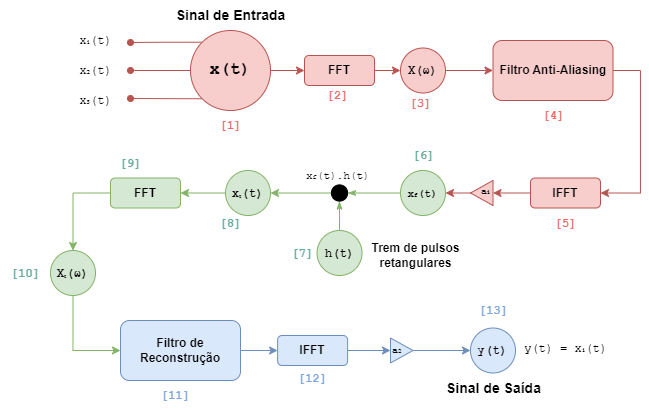
\includegraphics[width=9cm]{Diagrama_Geral.png} % leia abaixo
\caption{Diagrama geral do projeto.}
\end{figure}

Como é ilustrado pela figura acima, o diagrama é dividido em três setores caracterizados por suas respectivas cores. Em vermelho, encontra-se a etapa de filtragem do sinal de entrada. Em seguida, em verde, a etapa de amostragem. Por fim, em azul, a etapa de reconstrução de sinal. Esta diferenciação foi aplicada meramente para fins didáticos. 

\subsection{Filtragem do Sinal de Entrada}

\subsubsection{Sinal de Entrada}

O sinal de entrada$^{[1]}$ é formado a partir da soma de diferentes senóides com suas respectivas frequências. Tomando como exemplo o diagrama do projeto, a primeira senóide ($x_1$) é o sinal que se deseja filtrar, enquanto que as demais ($x_2$ e $x_3$) representam, neste caso, ruídos indesejáveis. 

\subsubsection{Sinal de Entrada na frequência}

Antes de filtrar o sinal de entrada, é necessário convertê-lo para o domínio da frequência. Para isto, pode-se utilizar a transformada rápida de fourier$^{[2]}$, representada pelo comando {\fontfamily{pcr}\selectfont fft} no Octave. Através dela, obtém-se o espectro de frequência do sinal, que é formado a partir de cada frequência das $n$ senóides que compõem $x(t)$.

\begin{figure}[H]
\captionsetup{justification=centering}
\centering % para centralizarmos a figura
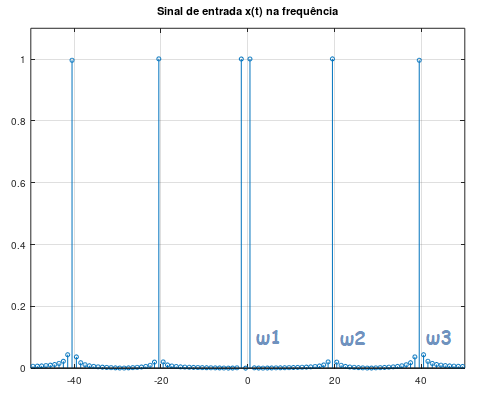
\includegraphics[width=4cm]{ex_sinal_entrada_freq.png} % leia abaixo
\caption{Componentes de frequência do sinal $x(t)$.}
\end{figure}

\subsubsection{Filtrando o Sinal de Entrada}

A fim de remover possíveis frequências indesejáveis, utiliza-se um filtro \textit{anti-aliasing} ideal$^{[4]}$. Matematicamente, este filtro nada mais é que uma função retangular de pulso único, representado no Octave pelo comando {\fontfamily{pcr}\selectfont rectpuls}. 

Efetuar um produto entre $X(\omega)$ e o filtro $rect(\omega)$ significa eliminar todas as frequências que não se encontram no intervalo definido pela área retangular. 

\begin{figure}[H]
\captionsetup{justification=centering}
\centering % para centralizarmos a figura
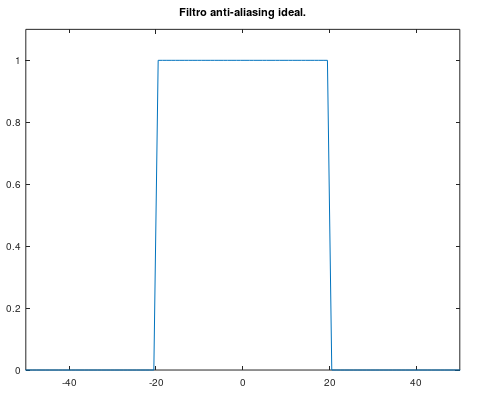
\includegraphics[width=3cm]{ex_filtro_aliasing.png} % leia abaixo
\caption{Exemplo de um filtro ideal $rect(\omega)$.}
\end{figure}

Quanto maior for a largura do pulso, mais informação do sinal original ele filtrará. Em outras palavras, se a largura do filtro tender ao infinito, todo o espectro de frequência será recuperado.

\begin{figure}[H]
\captionsetup{justification=centering}
\centering % para centralizarmos a figura
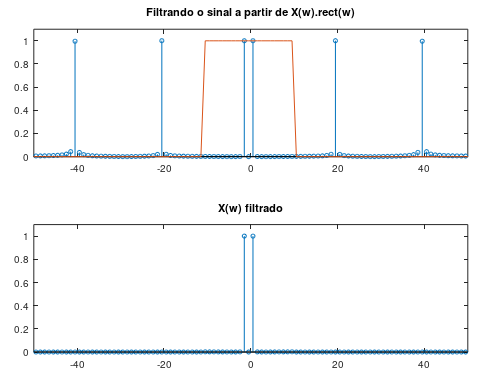
\includegraphics[width=4cm]{ex_filtrando.png} % leia abaixo
\caption{Representação gráfica do processo de filtragem. Nesta situação, a frequência $\omega$$_1$ foi filtrada.}
\end{figure}

\subsubsection{Retornando para o domínio do tempo}

Após filtrar o sinal, basta retornar para o domínio do tempo. Para isto, utiliza-se a transformada rápida inversa de fourier$^{[5]}$, cujo comando no Octave é {\fontfamily{pcr}\selectfont ifft}. Uma vez que o sinal de entrada filtrado $x$$_f$$(t)$ é reconstruído, o resultado gráfico no tempo deve ser semelhante a curva senoidal correspondente à frequência filtrada. Além disso, o processo de filtragem também gera atenuação na amplitude do sinal, portanto é necessário fazer uma amplificação no sinal $x$$_f$$(t)$ para uma melhor aproximação a senóide desejada.

\begin{figure}[H]
\captionsetup{justification=centering}
\centering % para centralizarmos a figura
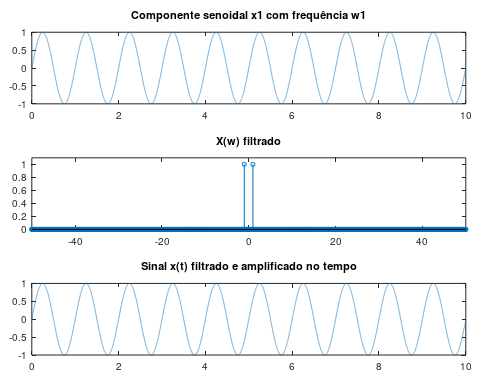
\includegraphics[width=4cm]{ex_amplificando.png} % leia abaixo
\caption{Comparação gráfica entre o componente senoidal $x_1$ e o sinal $x$$_f$$(t)$.}
\end{figure}

\subsection{Amostragem do Sinal}

\subsubsection{Trem de pulsos retangulares}

Seguindo a ordem estabelecida pelo diagrama, tem-se, enfim, o sinal filtrado$^{[6]}$ e pronto para ser amostrado. Este processo de amostragem é feito através de um PAM natural. Em outras palavras, efetua-se um produto do sinal $x$$_f$$(t)$ por um trem de pulsos retangulares$^{[7]}$ $h(t)$, cuja frequência $w$$_s$ equivale a taxa de amostragem. Portanto, esta deve ser, no mínimo, duas vezes a frequência $w$ (ou $w$$_1$) do sinal $x$$_f$$(t)$.

\begin{figure}[H]
\captionsetup{justification=centering}
\centering % para centralizarmos a figura
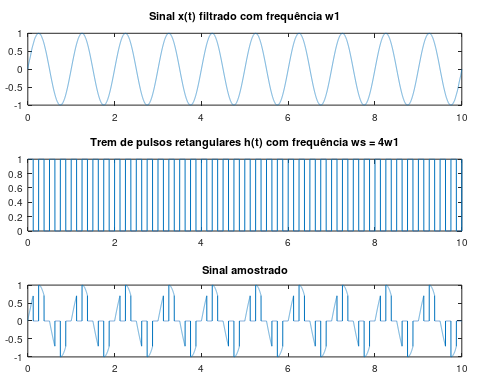
\includegraphics[width=4cm]{ex_amostrando.png} % leia abaixo
\caption{Obtenção do sinal amostrado $x$$_s$$(t)$ a partir de um sinal de pulsos retangulares $h(4w$$_1$$t)$.}
\end{figure}

\subsubsection{Replicação dos espectros}

Uma vez obtido o sinal amostrado$^{[8]}$ $x$$_s$$(t)$, deve-se novamente utilizar a FFT$^{[9]}$ para obter $X$$_s$$(\omega)$, e é neste ponto que ocorre o fenômeno da replicação dos espectros. Como a amostragem não é feita com impulsos ideais, as réplicas também não são ideias. Dessa forma, suas amplitudes são gradativamente atenuadas tendendo à zero.

\begin{figure}[H]
\captionsetup{justification=centering}
\centering % para centralizarmos a figura
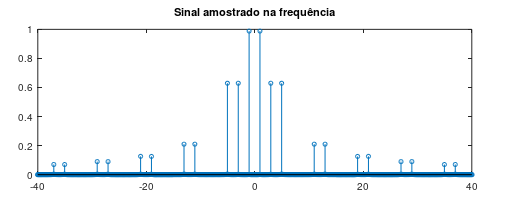
\includegraphics[width=4cm]{ex_replicacao.png} % leia abaixo
\caption{Sinal $x$$_s$$(t)$ na frequência. Com o gráfico ampliado, é possível perceber múltiplos pares de réplicas da frequência original, mas que são gradativamente atenuadas.}
\end{figure}

\subsection{Reconstrução do Sinal Amostrado}

\subsubsection{Filtro de reconstrução}

Através do sinal amostrado em frequência $X$$_s$$(\omega)$$^{[10]}$, o próximo passo, como o próprio diagrama ilustra, é aplicar um filtro de reconstrução$^{[11]}$ para obter a frequência original $w$$_1$ do sinal $x$$_f$$(t)$. Este processo não difere do já abordado filtro \textit{anti-aliasing}. Neste caso, o filtro ideal é aplicado no intervalo em que se encontra o espectro de frequência de interesse e tentando, o máximo possível, evitar réplicas parasitas.

\begin{figure}[H]
\captionsetup{justification=centering}
\centering % para centralizarmos a figura
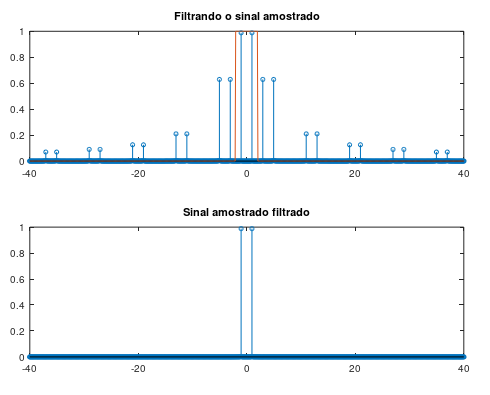
\includegraphics[width=4cm]{ex_filtrando_amostr.png} % leia abaixo
\caption{Filtro de recuperação (em laranja) aplicado em $X$$_s$$(\omega)$. No gráfico inferior, o sinal filtrado com o componente de frequência original $w$$_1$.}
\end{figure}

\subsubsection{Sinal recuperado}

Por fim, basta aplicar IFFT$^{[12]}$ em $X$$_s$$(\omega)$ filtrado para reconstruir o sinal $x$$_f$$(t)$. O resultado desta operação é a saída do sistema$^{[13]}$, que equivale a senóide $x$$_1$.

\begin{figure}[H]
\captionsetup{justification=centering}
\centering % para centralizarmos a figura
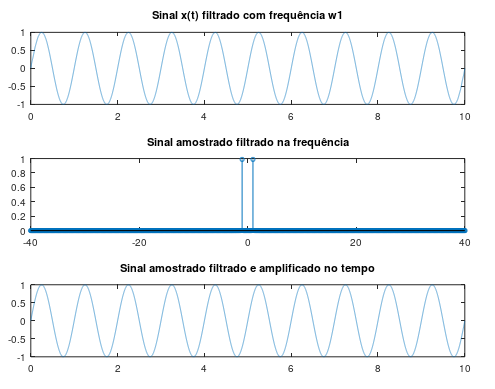
\includegraphics[width=4cm]{ex_amplificando_amostr.png} % leia abaixo
\caption{Comparação entre $x$$_f$$(t)$ com o sinal amostrado $x$$_s$$(t)$ após a filtragem e amplificação.}
\end{figure}

\section{Resultados e Discussões}
\section{Conclusão}

% references section

% can use a bibliography generated by BibTeX as a .bbl file
% BibTeX documentation can be easily obtained at:
% http://mirror.ctan.org/biblio/bibtex/contrib/doc/
% The IEEEtran BibTeX style support page is at:
% http://www.michaelshell.org/tex/ieeetran/bibtex/
%\bibliographystyle{IEEEtran}
% argument is your BibTeX string definitions and bibliography database(s)
%\bibliography{IEEEabrv,../bib/paper}
%
% <OR> manually copy in the resultant .bbl file
% set second argument of \begin to the number of references
% (used to reserve space for the reference number labels box)
\bibliographystyle{IEEEtran}
\bibliography{bibtex/bib/IEEEabrv,bibtex/bib/IEEEexample}

\end{document}
